\subsection{Summability Methods}

\begin{theorem} \label{thm:summation-by-parts} \hlt{Summation by Parts}\\
Given two sequences $(a_n)$ and $(b_n)$, put $A_n\defeq\sum\limits_{k=0}^{n}a_k$ and $A_{-1}\defeq0$.\\
If $0\leq p\leq q$, then $\sum\limits_{n=p}^{q}a_nb_n=\sum\limits_{n=p}^{q-1}A_n(b_n-b_{n+1})+A_qb_q-A_{p-1}b_p$.
\begin{proof}
Since $a_n=A_n-A_{n-1}$, $\sum\limits_{n=p}^{q}a_nb_n=\sum\limits_{n=p}^{q}A_nb_n-\sum\limits_{n=p}^{q}A_{n-1}b_n =\sum\limits_{n=p}^{q}A_nb_n-\sum\limits_{n=p-1}^{q-1}A_nb_{n+1}$.\\
\hlt{Structural Commentary}: This is the discrete analogue of integration by parts.\\
\hlt{Key Insight}: Move the difference from $a_n$ onto $b_n$ by rewriting $a_n=A_n-A_{n-1}$.
\end{proof}
\end{theorem}

\begin{theorem} \label{thm:dirichlet-test-series} \hlt{Dirichlet Test}\\
If the partial sums $A_n$ of $\sum a_n$ are bounded, $b_n\downarrow0$, and $b_n\geq0$, then $\sum a_nb_n$ converges.
\begin{proof}
Choose $M$ with $\abs{A_n}\leq M$. If $M=0$, the result is immediate. Otherwise choose $N$ with $b_N\leq\varepsilon/(2M)$.\\
For $N\leq p\leq q$, $\abs{\sum\limits_{n=p}^{q}a_nb_n}\leq M\left(\sum\limits_{n=p}^{q-1}(b_n-b_{n+1})+b_q+b_p\right)=2Mb_p\leq2Mb_N\leq\varepsilon$. Theorem \ref{thm:series-cauchy-criterion} applies.\\
\hlt{Structural Commentary}: Bounded oscillation in $A_n$ is damped by a monotone scalar tending to $0$.\\
\hlt{Key Insight}: Summation by parts converts cancellation into a total variation estimate for $b_n$.
\end{proof}
\end{theorem}

\begin{figure}[H]
  \centering
  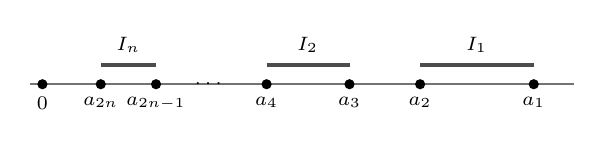
\begin{tikzpicture}[
  x=0.78cm,
  y=0.72cm,
  every node/.style={font=\scriptsize},
  axis/.style={black!55, line width=0.55pt},
  point/.style={circle, fill=black, inner sep=1.3pt},
  interval/.style={black!70, line width=1.2pt}
]
  \draw[axis] (-0.2,0) -- (8.65,0);

  \foreach \x/\lab in {
    0/$0$,
    0.95/a_{2n},
    1.85/a_{2n-1},
    3.65/a_4,
    5.00/a_3,
    6.15/a_2,
    8.00/a_1
  } {
    \node[point] at (\x,0) {};
    \node[below] at (\x,-0.05) {$\lab$};
  }

  \draw[interval] (0.95,0.34) -- (1.85,0.34);
  \draw[interval] (3.65,0.34) -- (5.00,0.34);
  \draw[interval] (6.15,0.34) -- (8.00,0.34);

  \node[above] at (1.40,0.38) {$I_n$};
  \node[above] at (4.32,0.38) {$I_2$};
  \node[above] at (7.07,0.38) {$I_1$};

  \node at (2.70,0) {$\cdots$};
\end{tikzpicture}

  \caption{The intervals $I_j=[a_{2j},a_{2j-1}]$ are disjoint inside $(0,a_1)$.}
  \label{fig:alternating-series-intervals}
\end{figure}

\begin{corollary} \label{cor:alternating-series-test} \hlt{Alternating Series Test}\\
Suppose $\abs{c_1}\geq\abs{c_2}\geq\abs{c_3}\geq\cdots$, the signs alternate, and $c_n\to0$. Then $\sum c_n$ converges.
\begin{proof}
After shifting indices to start at $0$ if desired, apply Theorem \ref{thm:dirichlet-test-series} with $a_n=(-1)^{n+1}$ and $b_n=\abs{c_n}$.\\
\hlt{Structural Commentary}: Alternation gives bounded sums; decreasing magnitudes damp them.\\
\hlt{Key Insight}: Alternating convergence is Dirichlet convergence in its simplest form.
\end{proof}
\end{corollary}

\begin{perspective} \label{per:alternating-series-interval-picture} \hlt{Alternating Partial Sums as Nested Control}\\
The interval picture explains the boundedness in Corollary \ref{cor:alternating-series-test}: the even partial sums collect disjoint lengths inside a fixed interval, while the odd partial sums differ from the even ones by the next term, which tends to $0$.
\end{perspective}

\begin{figure}[H]
  \centering
  \begin{tikzpicture}[
  >=Stealth,
  x=0.72cm,
  y=3.0cm,
  every node/.style={font=\scriptsize},
  axis/.style={->, gray!70, line width=0.55pt},
  odd/.style={blue!70!black, line width=0.9pt},
  even/.style={orange!85!black, line width=0.9pt},
  limit/.style={black!60, dashed, line width=0.6pt},
  pointodd/.style={circle, fill=blue!70!black, inner sep=1.35pt},
  pointeven/.style={circle, fill=orange!85!black, inner sep=1.35pt}
]
  \draw[axis] (0.35,0.43) -- (10.25,0.43) node[right] {$n$};
  \draw[axis] (0.7,0.43) -- (0.7,1.07) node[above] {$s_n$};
  \draw[limit] (0.82,0.693) -- (9.75,0.693)
    node[right, black] {$\log 2$};

  \draw[odd] plot coordinates {(1,1.000) (3,0.833) (5,0.783) (7,0.760) (9,0.746)};
  \draw[even] plot coordinates {(2,0.500) (4,0.583) (6,0.617) (8,0.635) (10,0.646)};

  \foreach \x/\y in {1/1.000,3/0.833,5/0.783,7/0.760,9/0.746} {
    \node[pointodd] at (\x,\y) {};
  }
  \foreach \x/\y in {2/0.500,4/0.583,6/0.617,8/0.635,10/0.646} {
    \node[pointeven] at (\x,\y) {};
  }
\end{tikzpicture}

  \caption{Odd partial sums (blue) decrease and even partial sums (orange) increase toward $\log2$.}
  \label{fig:alternating-harmonic-partial-sums}
\end{figure}

\begin{definition} \label{def:absolute-and-nonabsolute-convergence} \hlt{Absolute and Nonabsolute Convergence}\\
The series $\sum a_n$ \hlt{converges absolutely} if $\sum\abs{a_n}$ converges.\\
If $\sum a_n$ converges but $\sum\abs{a_n}$ diverges, then $\sum a_n$ converges \hlt{nonabsolutely}.
\end{definition}

\begin{theorem} \label{thm:absolute-convergence-implies-convergence} \hlt{Absolute Convergence Implies Convergence}\\
If $\sum a_n$ converges absolutely, then $\sum a_n$ converges.
\begin{proof}
For $m\geq n$, $\abs{\sum\limits_{k=n}^{m}a_k}\leq\sum\limits_{k=n}^{m}\abs{a_k}$. Apply Theorem \ref{thm:series-cauchy-criterion} to $\sum\abs{a_n}$.\\
\hlt{Structural Commentary}: Absolute convergence removes cancellation from the convergence question.\\
\hlt{Key Insight}: Small absolute tails force small signed or complex tails.
\end{proof}
\end{theorem}

\begin{theorem} \label{thm:linearity-of-convergent-series} \hlt{Addition and Scalar Multiplication of Series}\\
If $\sum a_n=A$ and $\sum b_n=B$, then $\sum(a_n+b_n)=A+B$ and $\sum ca_n=cA$ for every fixed scalar $c$.
\begin{proof}
Apply Theorem \ref{thm:complex-sequence-limit-algebra} to the corresponding partial sums.\\
\hlt{Structural Commentary}: Linearity of convergent series is just limit algebra for partial sums.\\
\hlt{Key Insight}: Add series by adding their partial-sum sequences.
\end{proof}
\end{theorem}

\begin{definition} \label{def:cauchy-product-of-series} \hlt{Cauchy Product}\\
Given $\sum a_n$, $\sum b_n$, define $c_n\defeq\sum\limits_{k=0}^{n}a_kb_{n-k}$, $(n=0,1,2,\ldots)$. Series $\sum c_n$ is \hlt{Cauchy product} of given series.
\end{definition}

\begin{figure}[H]
  \centering
  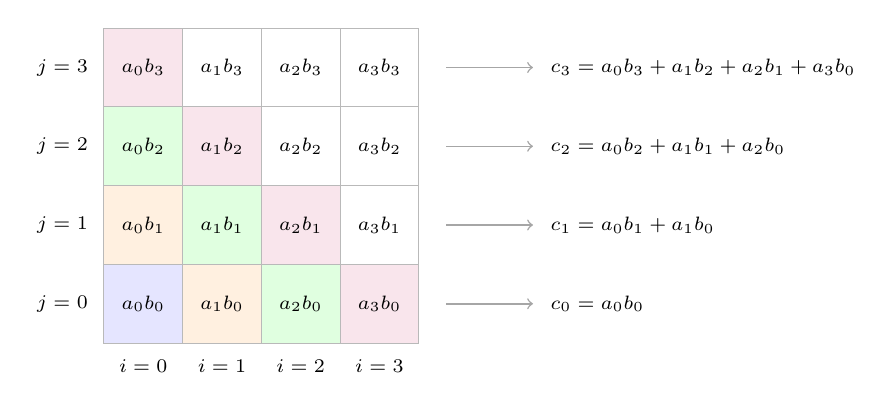
\begin{tikzpicture}[
  every node/.style={font=\scriptsize},
  cell/.style={draw=gray!55, line width=0.35pt},
  diagA/.style={fill=blue!10},
  diagB/.style={fill=orange!12},
  diagC/.style={fill=green!12},
  diagD/.style={fill=purple!10},
  arrow/.style={->, gray!70, line width=0.55pt}
]
  \foreach \i in {0,1,2,3} {
    \foreach \j in {0,1,2,3} {
      \pgfmathtruncatemacro{\diagindex}{\i+\j}
      \ifnum\diagindex=0
        \path[diagA] (\i,\j) rectangle ++(1,1);
      \fi
      \ifnum\diagindex=1
        \path[diagB] (\i,\j) rectangle ++(1,1);
      \fi
      \ifnum\diagindex=2
        \path[diagC] (\i,\j) rectangle ++(1,1);
      \fi
      \ifnum\diagindex=3
        \path[diagD] (\i,\j) rectangle ++(1,1);
      \fi
      \draw[cell] (\i,\j) rectangle ++(1,1);
      \node at (\i+0.5,\j+0.5) {$a_{\i}b_{\j}$};
    }
  }

  \foreach \i in {0,1,2,3} {
    \node[below] at (\i+0.5,-0.08) {$i=\i$};
    \node[left] at (-0.08,\i+0.5) {$j=\i$};
  }

  \draw[arrow] (4.35,0.5) -- (5.45,0.5);
  \node[right, align=left] at (5.55,0.5) {$c_0=a_0b_0$};

  \draw[arrow] (4.35,1.5) -- (5.45,1.5);
  \node[right, align=left] at (5.55,1.5) {$c_1=a_0b_1+a_1b_0$};

  \draw[arrow] (4.35,2.5) -- (5.45,2.5);
  \node[right, align=left] at (5.55,2.5) {$c_2=a_0b_2+a_1b_1+a_2b_0$};

  \draw[arrow] (4.35,3.5) -- (5.45,3.5);
  \node[right, align=left] at (5.55,3.5) {$c_3=a_0b_3+a_1b_2+a_2b_1+a_3b_0$};

\end{tikzpicture}

  \caption{Diagonal sums of $(a_i b_j)$ form the Cauchy product; finite rectangular sums are order-free.}
  \label{fig:cauchy-product-diagonals}
\end{figure}

\begin{perspective} \label{per:cauchy-product-diagonal-ordering} \hlt{Diagonal Ordering in a Product}\\
$c_n$ is the diagonal sum of the products $a_i b_j$ with $i+j=n$. Absolute convergence, as in Theorems \ref{thm:mertens-cauchy-product} and \ref{thm:absolute-convergence-rearrangements}, keeps the value independent of the accumulation order.
\end{perspective}

\begin{theorem} \label{thm:mertens-cauchy-product} \hlt{Mertens' Theorem for Cauchy Products}\\
Suppose $\sum a_n$ converges absolutely, $\sum a_n=A$, $\sum b_n=B$, and $c_n=\sum\limits_{k=0}^{n}a_kb_{n-k}$. Then $\sum\limits_{n=0}^{\infty}c_n=AB$.
\begin{proof}
Let $A_n,B_n,C_n$ be the partial sums and set $\beta_n\defeq B_n-B$.\\
Then $C_n=A_nB+\gamma_n$, and $\gamma_n\defeq a_0\beta_n+a_1\beta_{n-1}+\cdots+a_n\beta_0$. Since $A_nB\to AB$, it suffices to show $\gamma_n\to0$.\\
Put $\alpha\defeq\sum\abs{a_n}$. If $\abs{\beta_j}\leq\varepsilon$ for $j\geq N$, then $\abs{\gamma_n}\leq \abs{\beta_0a_n+\cdots+\beta_Na_{n-N}}+\varepsilon\alpha$.\\
Let $n\to\infty$ with $N$ fixed. The first term tends to $0$, so $\limsup\abs{\gamma_n}\leq\varepsilon\alpha$; let $\varepsilon\downarrow0$.\\
\hlt{Structural Commentary}: Absolute convergence of one factor controls the convolution error.\\
\hlt{Key Insight}: One absolute factor makes the Cauchy product converge to $AB$.
\end{proof}
\end{theorem}

\begin{definition} \label{def:series-rearrangement} \hlt{Rearrangement of a Series}\\
If $(k_n)$ lists each positive integer exactly once and $a'_n\defeq a_{k_n}$, then $\sum a'_n$ is a \hlt{rearrangement} of $\sum a_n$.
\end{definition}

\begin{theorem} \label{thm:riemann-rearrangement-theorem} \hlt{Riemann Rearrangement Theorem}\\
If real $\sum a_n$ converges nonabsolutely and $-\infty\leq\alpha\leq\beta\leq\infty$,\\
then some rearrangement has partial sums $s'_n$ with $\liminf\limits_{n\to\infty}s'_n=\alpha$ and $\limsup\limits_{n\to\infty}s'_n=\beta$.
\begin{proof}
Write $a_n=p_n-q_n$, where $p_n=\max(a_n,0)$ and $q_n=\max(-a_n,0)$. Since $\sum a_n$ converges but not absolutely, $\sum p_n=\sum q_n=+\infty$, and $p_n,q_n\to0$. List the positive nonzero $p_n$ as $P_1,P_2,\ldots$ and the positive nonzero $q_n$ as $Q_1,Q_2,\ldots$, preserving their original orders.\\
Choose finite numbers $\ell_N<u_N$ with $\ell_N\to\alpha$ and $u_N\to\beta$ in the extended sense. Starting from partial sum $0$, add unused $P$ terms until the sum is $>u_N$, then add unused terms $-Q$ until the sum is $<\ell_N$; repeat for $N=1,2,\ldots$. Divergence of both positive series makes each stopping time finite, and the alternating stages use every nonzero positive and negative term eventually. Insert zero terms anywhere.\\
After the $N$th upward crossing, the partial sum lies between $u_N$ and $u_N+P_j$ for the next positive term used; after the downward crossing, it lies between $\ell_N-Q_j$ and $\ell_N$ for the next negative term used. Since $P_j,Q_j\to0$, these overshoots vanish. Hence subsequences of partial sums approach the upper targets and lower targets, while all later partial sums stay within vanishing error of $[\ell_N,u_N]$. Therefore $\liminf s'_n=\alpha$ and $\limsup s'_n=\beta$.\\
\hlt{Structural Commentary}: Conditional convergence leaves enough mass to steer partial sums.\\
\hlt{Key Insight}: Vanishing terms make the steering increasingly precise.
\end{proof}
\end{theorem}

\begin{theorem} \label{thm:absolute-convergence-rearrangements} \hlt{Absolutely Convergent Series Are Rearrangement-Invariant}\\
Every rearrangement of an absolutely convergent complex series converges to the same sum.
\begin{proof}
Let $s_n,s'_n$ be the original and rearranged partial sums.\\
Given $\varepsilon>0$, choose $N$ so that $\sum_{i=N}^{m}\abs{a_i}\leq\varepsilon$ for $m\geq N$, then choose $p$ so $a_1,\ldots,a_N$ occur among $a'_1,\ldots,a'_p$.\\
For $n>p$, $s_n-s'_n$ uses only tail terms, hence $\abs{s_n-s'_n}\leq\varepsilon$. Thus $s'_n$ has the same limit as $s_n$.\\
\hlt{Structural Commentary}: Absolute tails control any finite reordering of the remaining terms.\\
\hlt{Key Insight}: Absolute convergence is exactly the protection needed against rearrangement.
\end{proof}
\end{theorem}

\begin{definition} \label{def:absolute-summation-over-countable-set} \hlt{Absolute Summation over Countable Sets}\\
Let $X$ be countable, $f:X\to\C$, and $g:\N\to X$ be a bijection, $g_n\defeq g(n)$.\\
If $\sum\limits_{n=1}^{\infty}\abs{f(g_n)}<\infty$, then $\sum\limits_{x\in X}f(x)$ is \hlt{absolutely convergent}, and $\sum\limits_{x\in X}f(x)\defeq\sum\limits_{n=1}^{\infty}f(g_n)$.
\end{definition}

\begin{theorem} \label{thm:absolute-countable-sums-well-defined} \hlt{Countable Sums Are Order-Free Under Absolute Convergence}\\
Let $X,Y$ be countable, $f:X\to\C$ be absolutely summable, and $h:Y\to X$ be a bijection.\\
Then $f\circ h$ is absolutely summable and $\sum\limits_{y\in Y}f(h(y))=\sum\limits_{x\in X}f(x)$.\\
In particular, a countable absolutely convergent sum is independent of the enumeration.
\begin{proof}
Let $g:\N\to X$ and $k:\N\to Y$ be enumerations, and set $\sigma\defeq g^{-1}\circ h\circ k:\N\to\N$.\\
Then $\sigma$ is a bijection and $h(k_n)=g_{\sigma(n)}$. Hence $\sum\limits_{n=1}^{\infty}\abs{f(h(k_n))} =\sum\limits_{n=1}^{\infty}\abs{f(g_{\sigma(n)})}<\infty$.\\
Thus $\sum\limits_{y\in Y}f(h(y)) =\sum\limits_{n=1}^{\infty}f(g_{\sigma(n)}) =\sum\limits_{n=1}^{\infty}f(g_n) =\sum\limits_{x\in X}f(x)$, where the middle equality is Theorem \ref{thm:absolute-convergence-rearrangements}.\\
Taking $Y=\N$ and $h$ to be any enumeration of $X$ gives enumeration independence.\\
\hlt{Structural Commentary}: Absolute convergence turns an enumeration into harmless bookkeeping.\\
\hlt{Key Insight}: Once absolute tails are controlled, the order of a countable listing no longer changes the sum.
\end{proof}
\end{theorem}

\begin{theorem} \label{thm:fubini-countable-absolute-series} \hlt{Fubini for Absolutely Summable Arrays}\\
Let $a_{mn}\in\C$ and suppose $L\defeq\sum\limits_{(m,n)\in\N\times\N}\abs{a_{mn}}<\infty$. Then each row and column is absolutely summable.\\
With $r_m\defeq\sum\limits_{n=1}^{\infty}a_{mn}$ and $c_n\defeq\sum\limits_{m=1}^{\infty}a_{mn}$, the row-total and column-total series are absolutely convergent,\\
where $\sum\limits_{m=1}^{\infty}\abs{r_m}<\infty$; $\sum\limits_{n=1}^{\infty}\abs{c_n}<\infty$, and $\sum\limits_{m=1}^{\infty}r_m =\sum\limits_{(m,n)\in\N\times\N}a_{mn} =\sum\limits_{n=1}^{\infty}c_n$.
\begin{proof}
For finite $F\subseteq\N\times\N$, $\sum_{(m,n)\in F}\abs{a_{mn}}\leq L$. Hence each row and column has bounded absolute partial sums, so rows and columns converge absolutely by Theorem \ref{thm:nonnegative-series-bounded-partial-sums}.\\
Moreover, for $M\geq1$, $\sum\limits_{m=1}^{M}\abs{r_m} \leq \sum\limits_{m=1}^{M}\sum\limits_{n=1}^{\infty}\abs{a_{mn}} =\lim\limits_{N\to\infty}\sum\limits_{m=1}^{M}\sum\limits_{n=1}^{N}\abs{a_{mn}} \leq L$, so $\sum\limits_m\abs{r_m}<\infty$.\\
Similarly $\sum\limits_n\abs{c_n}<\infty$. Let $\varepsilon>0$. Choose finite $F\subseteq\N\times\N$ with $\sum\limits_{(m,n)\in(\N\times\N)\setminus F}\abs{a_{mn}}<\varepsilon$, and choose a rectangle $R=\{1,\ldots,M\}\times\{1,\ldots,N\}\supseteq F$. The full sum, row-iterated sum, and column-iterated sum each differ from $\sum\limits_{(m,n)\in R}a_{mn}$ by at most $\sum\limits_{(m,n)\in(\N\times\N)\setminus R}\abs{a_{mn}}\leq\varepsilon$. Let $\varepsilon\downarrow0$.\\
\hlt{Structural Commentary}: Finite rectangles plus absolute tails justify Fubini.\\
\hlt{Key Insight}: Double sums can be rearranged only after the entire array is absolutely summable.
\end{proof}
\end{theorem}

\begin{method} \label{meth:series-proof-patterns-source-todo}\label{meth:series-proof-patterns} \hlt{Series Proof Patterns}
\begin{enumerate}[label=(\roman*)]
\setlength{\itemsep}{0pt}
\item \hlt{Partial sums}: translate every assertion about $\sum a_n$ into an assertion about $s_n=\sum_{k=1}^{n}a_k$.
\item \hlt{Cauchy tails}: prove convergence by estimating $\abs{\sum_{k=n}^{m}a_k}$ for $m\geq n$.
\item \hlt{Nonnegative terms}: replace convergence by boundedness of partial sums.
\item \hlt{Comparison}: dominate only the tail; finitely many early terms are irrelevant.
\item \hlt{Absolute convergence}: use $\sum\abs{a_n}$ when cancellation should not matter.
\item \hlt{Countable index sets}: choose a bijection $g:\N\to X$; use Theorem \ref{thm:absolute-countable-sums-well-defined} so $\sum_{x\in X}a_x$ is independent of $g$.
\item \hlt{Double sums}: prove identities on $R_{M,N}\defeq\{1,\ldots,M\}\times\{1,\ldots,N\}$; pass to $\infty$ arrays (Theorem \ref{thm:fubini-countable-absolute-series}).
\item \hlt{Conditional convergence}: order matters; use summation by parts or rearrangements.
\end{enumerate}
\hlt{Key Insight}: Series arguments are sequence arguments with special notation for tails.
\end{method}
